\section{Cylc Introduction}


\subsection{The suite.rc File}

A cylc suite is a collection of files in a {\em suite directory} configured by
a single {\em suite.rc} file, which is written in a nested INI format with
section and sub-section headings denoted by square brackets.

\begin{lstlisting}[language=suiterc]
[section]
    option = value
    [[sub-section]]
        option = value
        [[[sub-sub-section]]]
            option = value
\end{lstlisting}

The most important top level sections in a suite.rc file are:

\begin{tabular}{ll}
\begin{lstlisting}
[cylc]
\end{lstlisting} & various suite-level configuration\\
\begin{lstlisting}
[scheduling]
\end{lstlisting} & determines when tasks are ready to run (dependencies etc.)\\
\begin{lstlisting}
[runtime]
\end{lstlisting} & defines {\em what} to run when a task is ready, and
where and how to run it \\
\end{tabular}


\subsection{Hello World in cylc}

This suite runs a single task named \lstinline{hello} that prints ``Hello
World!'' to standard out and then sleeps for 30 seconds before exiting.

% Call task "hello" to distinguish task name from suite name.
% Sleep for 30 seconds - long enough to be seen in the GUI.

\begin{lstlisting}[language=suiterc]
[scheduling]
    [[dependencies]]
        graph = hello
[runtime]
    [[hello]]
        script = echo "Hello World!"; sleep 30
\end{lstlisting}

The \lstinline{[scheduling]} section tells cylc to run the hello task
immediately on start-up (because it does not depend on other tasks and has no
clock triggers).  The \lstinline=[runtime]= section configures cylc to 
run the inlined ``Hello World!'' shell scripting for the task (as a background
job on the suite host, by default).  Section~\ref{Tasks} below explains how
this works.

\more{This isn't quite the simplest possible cylc suite. You can omit the runtime
configuration for a task and cylc will automatically create a minimal dummy job
for it. This can be useful for mocking up suites, and temporarily "dummying
out" real tasks}.

Here's how to run a new suite (don't do this yet; see below):

\begin{lstlisting}[language=bash]
$ cylc register hello_world /path/to/suite/
$ cylc validate hello_world
$ cylc run hello_world
\end{lstlisting}

\more{
    \begin{itemize}
        \item
    \lstinline{cylc-register} just associates a name with a suite definition.
    Commands that parse a suite can refer to this suite name or the file path;
    commands that connect to a suite daemon must refer to the suite name.

        \item
    \lstinline{cylc validate} checks for errors in the suite.rc file.

        \item
    \lstinline{cylc run} starts a server program to manage your workflow. It
    {\em daemonizes} (by default) and will stay alive if you log out. If your
    suite runs to completion, it will automatically shut down.
    \end{itemize}
}

\textcolor{red}{For this tutorial, however, we will be using the
\lstinline{rose suite-run} command to run suites}.  It automatically installs,
registers, validates, starts the suite, and opens the cylc GUI.  Rose
is installed on your metomi VM. 

\more{ \lstinline{rose suite-run} will soon be migrated into cylc.  It is a
    convenient short-cut command, but more importantly it {\em installs} the
    suite into its run directory and registers it there.  This separates the
    live suite from its source, and provides an opportunity to install external
files into the suite at start-up.  }

\paragraph*{Demo}
Copy the ``hello world example'' into a suite.rc file in a directory called
hello\_world, and run the following commands:

\begin{lstlisting}[language=bash]
$ cd hello_world
$ touch rose-suite.conf  # create an empty rose-suite.conf file
$ rose suite-run  # run the suite
\end{lstlisting}

If successful cylc will generate some output and open the cylc monitoring and
control GUI, which displays the current status of your suite. You should
briefly see the task \lstinline{hello_world} displayed with a coloured square
that represents its state. For example green means the task is running and gray
that it has succeeded.  Once the task has succeeded, the suite has no more
tasks to run and will automatically shut down.

The task job script and its standard out and standard error are captured to
a standard log directory location:
\begin{lstlisting}[language=bash]
$ ls -1 $HOME/cylc-run/hello_world/log/job/1/hello/01/
job
job.out
job.err
job.status
job-activity.log
\end{lstlisting}

\more{The directory path contains the suite name (hello\_world), log type
    ({\em job} or {\em suite}), task cycle point (1 for a non-cycling
    suite), task name (hello), and task submit number (01). This avoids
    unmanagably large flat log directories, and job logs don't get
overwritten even if tasks are resubmitted.}

While a task is still visible in the GUI you can right-click on it to view its
log files.  After that, look in its log directory,

\begin{lstlisting}[language=bash]
$ cd $HOME/cylc-run/hello_world/log/job/1/hello/01/
$ cat job.out
\end{lstlisting}

or use the \lstinline{cylc cat-log} command (which knows the file's location),

\begin{lstlisting}[language=bash]
$ cylc cat-log --help  # see "cylc --help" for top level command help
$ cylc cat-log --stdout hello_world hello.1
...
Hello World!
...
\end{lstlisting}

or use the fantastic \lstinline{rose suite-log} web suite log file viewer.

\begin{lstlisting}[language=bash]
$ cd hello_world
$ rose suite-log
\end{lstlisting}

\more{
    The \lstinline{rose suite-log} viewer will also be migrated to the cylc
    project soon.
}

\subsection{Tasks}
\label{Tasks}

Any program or script can be used as a cylc task without modification so long as,
\begin{itemize}
    \item it waits on any internal processes before returning (e.g.\ jobs
        submitted internally to a batch scheduler)
    \item it returns standard shell exit status: zero for success, non-zero
        for error (use \lstinline{set -e} in scripts)
\end{itemize}

\more{Cylc automatically wraps jobs in scripting that traps errors, directs
    job standard output and error to log files, and automatically communicates
    progress to the parent suite daemon. These {\em job scripts} can be found
in the task job log directory.}

A task job can run shell scripting inlined in the suite.rc file, or an
external program or script, or any combination of the two.  A suite
sub-directory called \lstinline{bin} is automatically added to your shell
\lstinline{$PATH} so that scripts residing in it can be called by name,

% changed original script name 'get-host-details' - users may wonder if host
% details are somehow communicated back to the suite.
\begin{lstlisting}[language=suiterc]
[runtime]
    [[model]]
        script = run-model
\end{lstlisting}

Alternatively, you can use a specify a full path,

\begin{lstlisting}[language=suiterc]
[runtime]
    [[model]]
        script = /path/to/my-scripts/run-model
\end{lstlisting}

or you can configure \lstinline{$PATH} in the task's environment,
\begin{lstlisting}[language=suiterc]
[runtime]
    [[model]]
        script = run-model
        [[[environment]]]
            PATH = /path/to/my-scripts:$PATH
\end{lstlisting}

\more{The last method makes more sense if there are multiple task scripts in
    the same location, then you can set \lstinline{$PATH} once in a {\em
    family} (see below) inherited by all the tasks
that need those scripts.}

An optional \lstinline=[[[remote]]]= sub-section determines {\em where} a task
will run (defaults to localhost), 

\begin{lstlisting}[language=suiterc]
[runtime]
    [[model]]
        script = run-model
        [[[remote]]]
            host = supercomputer
\end{lstlisting}

\more{Cylc doesn't install files to remote hosts for you.  If a task host does
    not share a filesystem with the suite host, make sure you install any files
    needed by the tasks that run there.  Rose (\ref{Rose}) can help automate
file installation.}

An optional \lstinline=[[[job]]]= sub-section determines {\em how} to run the
task (default to a shell "background" subprocess).
\begin{lstlisting}[language=suiterc]
[runtime]
    [[model]]
        script = run-model
        [[[remote]]]
            host = supercomputer
        [[[job]]]
            batch system = pbs
\end{lstlisting}

\more{Cylc can submit jobs to various batch systems such as PBS and SLURM. With
    these you generally have to use a \lstinline=[[[directives]]]=
    section too, to set the queue, wall clock limit, and so on.}

You can pass information to a script via its command line or environment,

\begin{lstlisting}[language=suiterc]
[runtime]
    [[model]]
        script = run-model --color=green
        [[[environment]]]
            START_TIME = $CYLC_TASK_CYCLE_POINT
\end{lstlisting}

For anything more complicated use custom scripting as you like (or an external
wrapper script),
\begin{lstlisting}[language=suiterc]
[runtime]
    [[model]]
        script = """
cat > model-input.txt <<__EOF__
COLOR=GREEN
START_TIME=$CYLC_TASK_CYCLE_POINT
__EOF__
run-model model-input.txt"""
\end{lstlisting}

Note that multi-line strings in the suite.rc file must be enclosed in triple
quotes.

\subsection{Graphs}

The hello\_world suite contained the line
\lstinline{graph = hello_world}. This is a graph string. In cylc
graph strings contain the logic for determining when tasks can be run. A graph
string should contain a list of tasks along with the inter-dependence between
them. For instance if we have two tasks \lstinline{foo} and \lstinline{bar},
where \lstinline{foo} is dependent on \lstinline{bar} succeeding, then we
would this logic in a graph string as:

\begin{lstlisting}[language=suiterc]
graph = foo => bar
\end{lstlisting}

This graph string tells cylc to run \lstinline{foo} and then once
\lstinline{foo} has succeeded run \lstinline{bar}. Note that if
\lstinline{foo} fails \lstinline{bar} will not run. These relationships are
called dependencies, a graph string can contain multiple dependencies.

\begin{lstlisting}[language=suiterc]
graph = """
    foo => bar
    bar => baz
    bar => qux
    baz => pin
    qux => pin
    wol
"""
\end{lstlisting}

\note{The graph string can be written over multiple lines using
triple, double quotation marks (\lstinline="""=).}

The logic of the previous graph string is outlined in the following diagram.

\begin{center}
    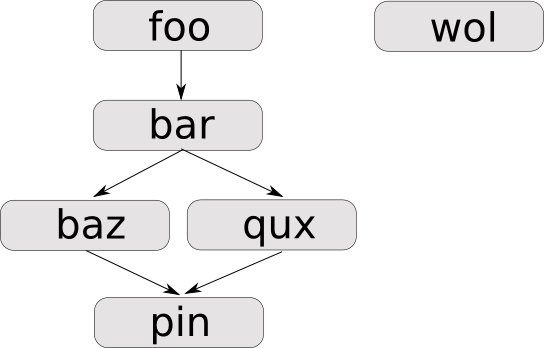
\includegraphics[width=0.4\columnwidth]{resources/tex/cylc-graph}
\end{center}


\subsection{Cycling}

Graph strings allow us to define workflows consisting of tasks. In a suite we
may well want to repeat workflows, which is called cycling.

\begin{center}
    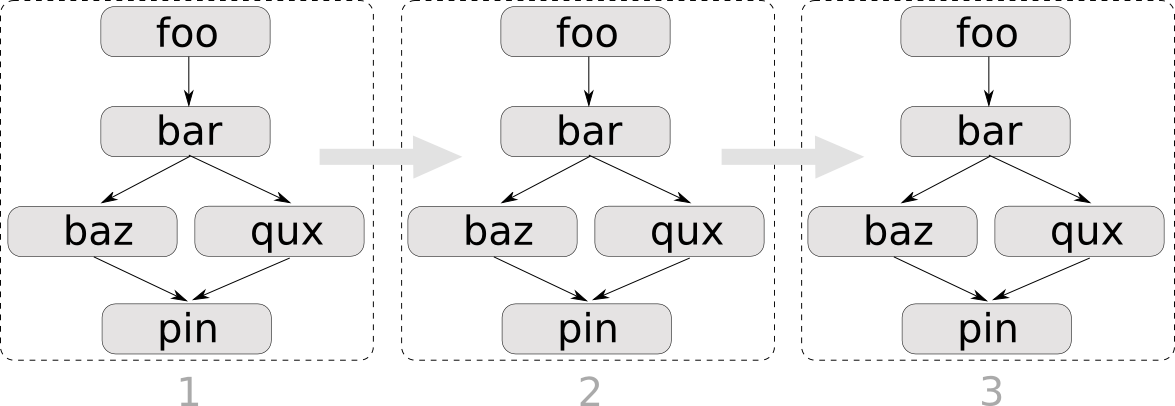
\includegraphics[width=0.6\columnwidth]{resources/tex/cylc-cycle-graph}
\end{center}

The above diagram shows the workflow from the previous example repeated three
times with the resultant cycles numbered 1, 2 and 3. With cylc cycles can
either be numbered or alternatively can use datetimes, for this tutorial shall
use datetimes.

In order to cycle a workflow we need a start point to begin cycling from, and
end point to finish cycling at. In cylc these are defined using the
\lstinline=initial cycle point= and \lstinline=final cycle point= values which
are set in the \lstinline=[scheduling]= section.

We tell cylc to cycle over a workflow using graph section headings. A graph
section heading is a section that sits inside the
\lstinline=[[dependencies]]= section. In the following example the task
\lstinline{foo} will run once every day at midday starting on the 1st of
January 2000 and ending on the 5th of January 2000.

\begin{lstlisting}[language=suiterc]
[scheduling]
    initial cycle point = 2000-01-01T00
    final cycle point = 2000-01-05T00
    [[dependencies]]
        [[[T12]]]
            graph = foo
\end{lstlisting}

In this example the graph section heading \lstinline=[[[T12]]]= means run
the workflow defined in the \lstinline=graph= section once every day at
12:00. Equally \lstinline=[[[T06]]]= means run every day at 06:00 and
\lstinline=[[[T2145]]]= means run every day at 21:45.

\note{When we talk of tasks running every day we don't mean that
the suite waits an entire day before running the next task, cycle points are
just labels we can use to organise cycles. It is possible to set real-world
datetimes as dependencies for cylc tasks see section
\ref{clock-triggered-tasks}.}

There are multiple forms of graph section heading to serve different purposes,
more exotic forms are outlined in section \ref{advanced-cycling}.


\subsection{Inter Cycle Dependence}

In the previous example the task \lstinline{foo} ran once every day. Because
we have not specified any dependencies multiple \lstinline{foo} tasks can end
up running in parallel. In order to make these tasks run one after the other
we will have to specify a dependency across cycle points as in the following
example:

\begin{lstlisting}[language=suiterc]
[scheduling]
    initial cycle point = 2000-01-01T00
    final cycle point = 2000-01-05T00
    [[dependencies]]
        [[[T12]]]
        graph = foo[-P1D] => foo
\end{lstlisting}

The expression \lstinline{foo[-P1D]} means \lstinline{foo} at a cycle point
one day earlier, hence in this example \lstinline{foo} will only run once
its previous run has succeeded. \lstinline{P1D} is an ISO8601 duration (for
details see \url{http://wikipedia.org/wiki/ISO_8601#Durations}), \lstinline=P=
denotes a duration and the \lstinline=1D= part means one day. The minus implies
that the duration is negative (going backwards in time), other examples of
ISO8601 durations are:

\begin{itemize}
    \item \lstinline{-PT12H} (12 hours ago).
    \item \lstinline{-PT6H30M} (6 hours 30 minutes ago).
    \item \lstinline{P1W} (1 week in the future).
\end{itemize}

\paragraph*{Demo}
This demo is an example of a cycling workflow, to run it create a new
directory and create a blank rose-suite.conf file within it.

Next copy the following code into a suite.rc and a bin/count-down file.

\begin{lstlisting}[language=]
|-- bin/
|   `-- count-down
|-- rose-suite.conf
`-- suite.rc
\end{lstlisting}

\begin{lstlisting}[language=suiterc, title=suite.rc]
[scheduling]
    initial cycle point = 2000-01-01T00
    final cycle point = 2000-01-05T00
    [[dependencies]]
        [[[T00]]]
            graph = """
                blast_off[-P1D] => point_upwards
                point_upwards => load_astronauts
                point_upwards => fill_fuel_tank
                point_upwards => set_coordinates
                fill_fuel_tank => light_fuse
                set_coordinates => count_down
                light_fuse => count_down
                load_astronauts => count_down
                count_down => blast_off
            """
[runtime]
    [[point_upwards]]
        script = sleep 2; echo "spikey end pointing at sky, flamey end \
                    pointing at ground"
    [[load_astronauts]]
        script = sleep 1; echo "loaded astronauts"
    [[fill_fuel_tank]]
        script = sleep 5; echo "tank brimmed"
    [[set_coordinates]]
        script = echo "coordinates set for west wallaby st"
    [[light_fuse]]
        script = echo "stand well back"
    [[count_down]]
        script = count-down
    [[blast_off]]
        script = echo "blast off"
\end{lstlisting}

\begin{lstlisting}[language=bash, title=bin/count-down]
sleep 1; echo 5;
sleep 1; echo 4;
sleep 1; echo 3;
sleep 1; echo 2;
sleep 1; echo 1;
\end{lstlisting}

To run this demo suite, enter the following commands:

\begin{lstlisting}[language=bash]
$ chmod +x bin/count-down  # Make the count-down script executable.
$ rose suite-run
\end{lstlisting}

Again a window should open up showing you the progress of the suite.
Whilst the suite is running try entering graph mode by selecting
\lstinline[language=]{View > 1 - Graph View} from the menubar, this will show
the dependencies between the tasks as they run.
